\section{Chapel Zippered Iteration}\label{sec:zippered_iteration}

Iteration is a widely used language feature in the Chapel programming language. Chapel iterators are blocks of code that are similar to functions and methods except that iterators can return multiple values back to the call site with the use of the \textit{yield} keyword instead of \textit{return}. Iterators are commonly used in loops to traverse data structures in a particular fashion. For example, an iterator $fibonacci(n: int)$ might be responsible for yielding the first $n$ Fibonacci numbers. This iterator could then be called in a loop's header to execute iterations 0, 1, 1, 2, 3, ... Arrays in Chapel support iteration by default. 

Chapel allows multiple iterators of the same size and shape to be iterated through simultaneously. This is known as \textit{zippered iteration} \cite{chamberlain2011user}. When zippered iteration is used, correpsonding iterations are processed together. On each loop iteration, an $n$-tuple is generated, where $n$ is the number of items in the zippering. The $d^{th}$ component of the tuple generated on loop iteration $j$ is the $j^{th}$ item that would be yielded by iterator $d$ in the zippering. Figure~\ref{zippered_iteration} shows an example of zippered iteration used in a Chapel \textbf{for} loop. 

Zippered iteration can be used with either sequential \textbf{for} loops or parallel \textbf{forall} loops in Chapel. Parallel zippered iteration is implemented in Chapel using leader-follower semantics. That is, a leader iterator is responsible for creating tasks and dividing up the work to carry out the parallelism. A follower iterator performs the work specified by the leader iterator for each task. Follower iterators generally resemble  serial iterators such as $fibonacci(n : int)$ shown in Figure \ref{zippered_iteration}a.

\subsection{Chapel Array Slicing}\label{sec:array_slicing}

Chapel supports another useful language feature known as \textit{array slicing}. This feature allows portions of an array to be accessed and modified in a succicnt fashion. For example, consider two arrays $A$ and $B$ containing indices from $1..10$. Suppose we wanted to assign elements $A[6]$, $A[7]$, and $A[8]$ to elements $B[1]$, $B[2]$, and $B[3]$ respectively. We could achieve this in one statement by writing $B[1..3] = A[6..8]$. Here, $A[6..8]$ is a slice of the original array $A$, and $B[1..3]$ is a slice of the original array $B$. An array slice can support a range of elements with a stride in some cases. For example, in the previous example, we could have made the assignment $B[1..3] = A[1..6$  $by$  $2]$. This would have assigned elements $A[1]$, $A[3]$, and $A[5]$ to elements $B[1]$, $B[2]$, and $B[3]$ respectively. Since all array slices in Chapel are arrays themselves, array slices are also iterable. 

Together, array slicing and parallel zippered iteration can express any parallel affine loop in Chapel that uses affine array accesses. Consider the code fragment in Figure \ref{affine_loop}a. There are two affine array accesses $A[i]$ and $B[i+2]$ in Figure \ref{affine_loop}a. The loop is written in a standard way where the loop induction variable $i$ takes on values from 1 to 10. Because the loop is a \textbf{forall} loop, loop iterations are not guaranteed to complete in a specific order. This loop assigns to elements of array $B$ to $A$ such that the $i^{th}$ element of $A$ is equal to the $(i+2)^{th}$ element of $B$ after the loop finishes. In Figure \ref{affine_loop}b, the same loop is written using zippered iteration. The loop induction variable $i$ no longer needs to be specifed, and each affine array access has been replaced with an array slice in the zippering of the loop header. It is possible to transform an affine loop in this fashion even when an affine array access has a constant factor multiplied by the loop induction variable. The resulting array slice will contain a stride equal to the constant factor.\footnote{Question by Aroon: Is it true to say that any affine array access can be transformed using the way described here? What if the access was something like $A[2i+3j]$?}

Because any parallel affine loop can be transformed to an equivalent parallel loop that uses zippered iteration, we observe a natural place in the Chapel programming language in which to implement modulo unrolling: the leader and follower iterators of the Cyclic and Block Cyclic distribution. 



\begin{figure}
	\begin{center}
	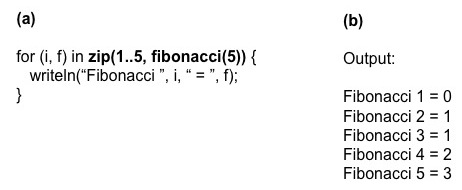
\includegraphics[scale=0.50]{./Figures/zippered_iteration}
	\caption{(a) Chapel code fragment showing a loop using zippered iteration. A tuple of loop index variables equal to the number of items in the zippering is declared in the loop header. If the variable $j$ corresponds to the current loop iteration, $i$ corresponds to the $j^{th}$ element in the range $1..5$, and $f$ corresponds to the $j^{th}$ element in the iterator $fibonacci(5)$. The \textit{zip} keyword tells the loop header which items to iterate over using zippered iteration. (b) Program output of the code fragment in Figure~\ref{zippered_iteration}a.}
	\label{zippered_iteration}
	\end{center}
\end{figure}

\begin{figure}
	\begin{center}
	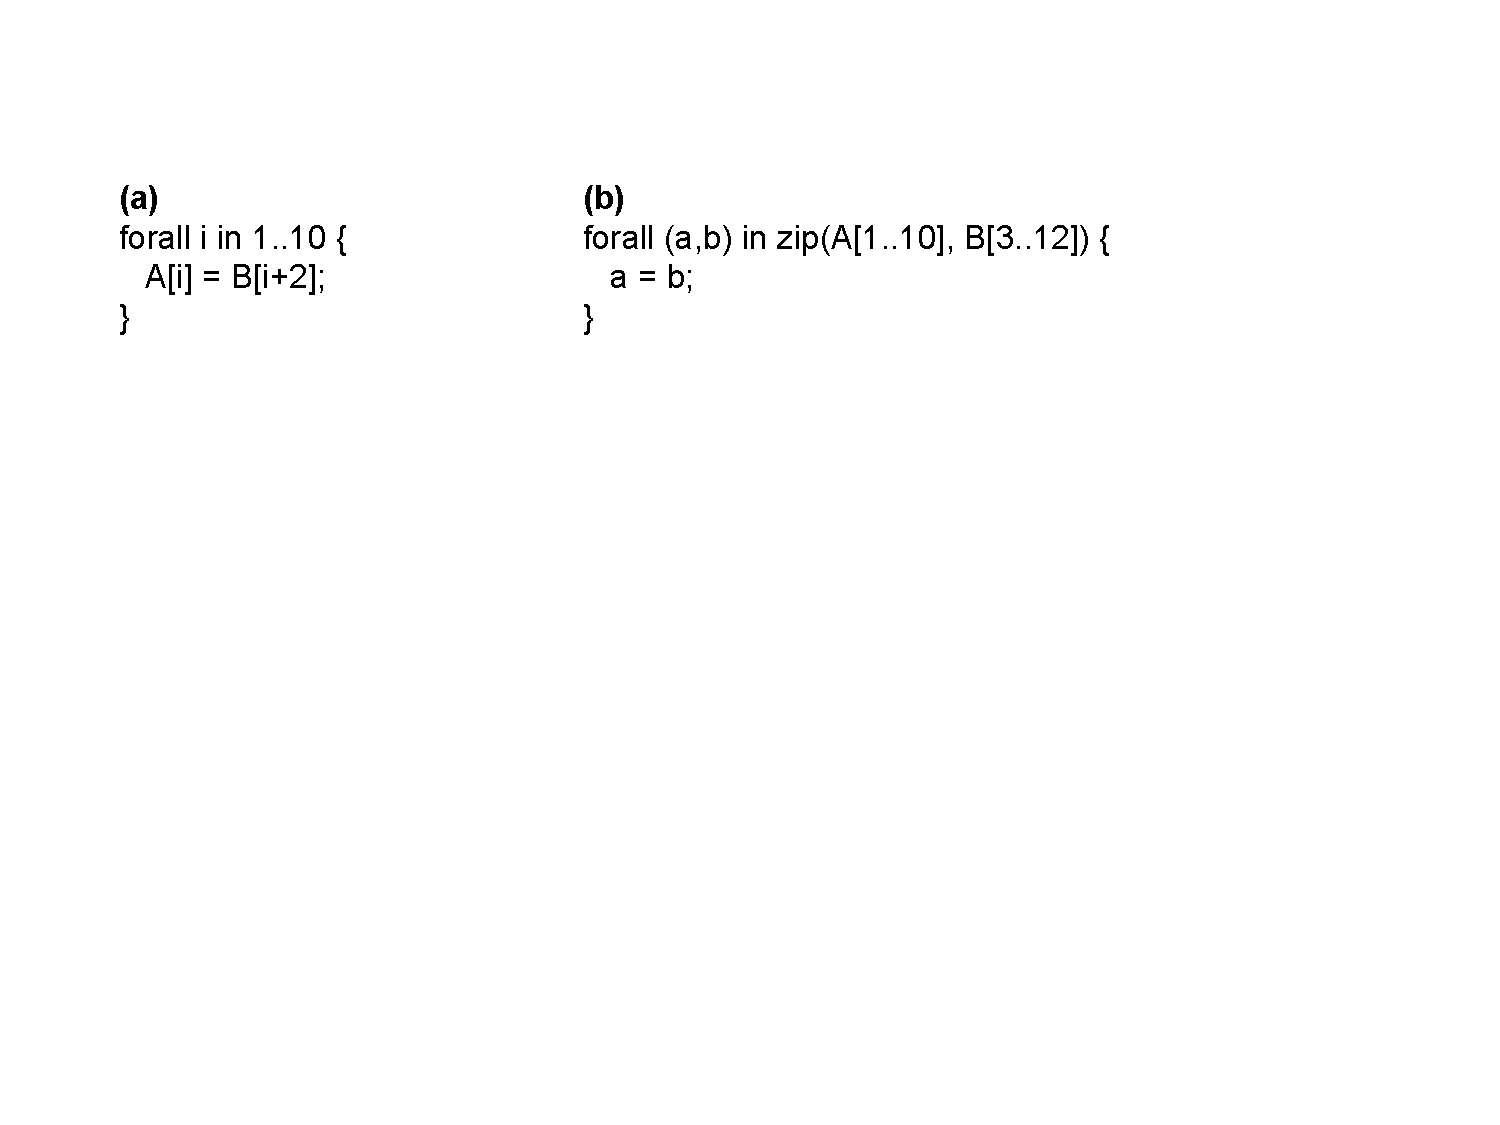
\includegraphics[scale=0.50]{./Figures/affine_loop}
	\caption{(a) Original loop written using a single loop induction variable $i$ ranging from 1 to 10. (b) The same loop written using zippered iteration. Instead of a loop induction variable and a range of values to denote the loop bounds, two array slices containing 10 elements each are specified.}
	\label{affine_loop}
	\end{center}
\end{figure}